\documentclass[11pt,a4paper]{report}
\usepackage[margin=1in]{geometry}
\usepackage[T1]{fontenc}
\usepackage{lmodern}
\usepackage{hyperref}
\usepackage{booktabs}
\usepackage{longtable}
\usepackage{listings}
\usepackage{xcolor}
\usepackage{graphicx}
\usepackage{tikz}
\usetikzlibrary{shapes,arrows.meta,positioning}

\hypersetup{colorlinks=true,linkcolor=blue,urlcolor=blue}
\lstdefinestyle{bash}{
  basicstyle=\ttfamily\small,
  breaklines=true,
  frame=single,
  backgroundcolor=\color{gray!8}
}
\lstdefinestyle{graphql}{
  basicstyle=\ttfamily\small,
  breaklines=true,
  frame=single,
  backgroundcolor=\color{gray!8}
}

\title{CXR GraphQL Lab Manual\\
\large SW.15 --- Apollo Gateway + federated mock services}
\author{CXR Ops Lab --- \texttt{cxr-ops-lab}}
\date{2026-05-31}

\begin{document}
\maketitle
\begin{abstract}
\textbf{SW.15}: Apollo \textbf{Gateway (:4000)} composes two subgraphs ---
\textbf{claims (:4001)} with CXR-shaped \texttt{Claim} types and
\textbf{policies (:4002)} with mock \texttt{Policy} lookups.
Standalone lab; \textbf{Claim Studio (:3000)} remains REST.
\end{abstract}
\tableofcontents
\newpage

\chapter{Architecture}

\begin{center}
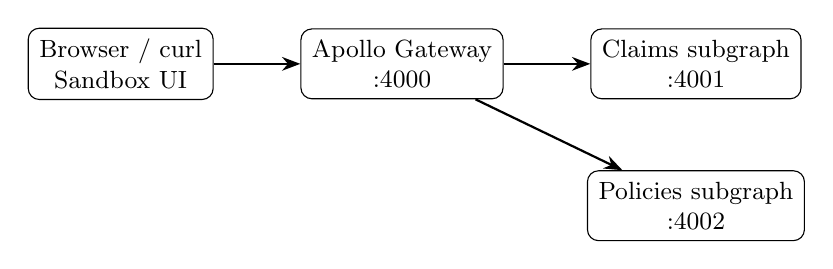
\begin{tikzpicture}[
  node distance=0.65cm and 0.5cm,
  box/.style={draw, rounded corners, minimum height=0.75cm, align=center, font=\small, inner sep=4pt},
  arr/.style={-{Stealth}, thick}
]
  \node[box] (br) {Browser / curl\\Sandbox UI};
  \node[box, right=1.1cm of br] (gw) {Apollo Gateway\\:4000};
  \node[box, right=1.1cm of gw] (cl) {Claims subgraph\\:4001};
  \node[box, below=0.9cm of cl] (po) {Policies subgraph\\:4002};
  \draw[arr] (br) -- (gw);
  \draw[arr] (gw) -- (cl);
  \draw[arr] (gw) -- (po);
\end{tikzpicture}
\end{center}

\chapter{CXR types (syllabus)}

\section{Claim (claims subgraph)}
\begin{lstlisting}[style=graphql]
type Claim {
  id: ID!
  status: String!
  summary: String
}
\end{lstlisting}
Fixtures: \texttt{demo-1} (status \texttt{ok}), \texttt{demo-2} (status \texttt{review}).

\section{Policy (policies subgraph)}
\begin{lstlisting}[style=graphql]
type Policy {
  id: ID!
  claimId: ID!
  code: String!
  description: String
}
\end{lstlisting}
\texttt{policyForClaim(claimId: "demo-1")} $\rightarrow$ \texttt{CXR-POL-OK}.

\chapter{Procedure}

\section{Start stack}
\begin{lstlisting}[style=bash]
cd cxr-ops-lab
./scripts/18-graphql-up.sh
./scripts/18-graphql-smoke.sh
\end{lstlisting}

\section{Browser golden path}
\begin{enumerate}
  \item Open \url{http://localhost:4000/graphql} (Apollo Sandbox).
  \item Paste query from \texttt{lab/graphql/query-golden.graphql}.
  \item Expect \texttt{claim.status = ok} and \texttt{policyForClaim.code = CXR-POL-OK}.
  \item Screenshot \texttt{evidence/SW15-graphql-sandbox-*.png} (optional).
\end{enumerate}

\chapter{File inventory}

\begin{longtable}{@{}p{5cm}p{8cm}@{}}
\toprule
File & Purpose \\
\midrule
\endhead
\texttt{compose.graphql.yaml} & Docker Compose for gateway + subgraphs \\
\texttt{lab/graphql/Dockerfile} & Node 20 image \\
\texttt{lab/graphql/claims-subgraph.mjs} & Federated claims service \\
\texttt{lab/graphql/policies-subgraph.mjs} & Federated policies service \\
\texttt{lab/graphql/gateway.mjs} & \texttt{IntrospectAndCompose} gateway \\
\texttt{lab/graphql/schema.graphql} & Composed schema reference \\
\texttt{lab/graphql/query-golden.graphql} & Golden path query \\
\texttt{scripts/18-graphql-up.sh} & Build + start \\
\texttt{scripts/18-graphql-smoke.sh} & Subgraph + federated probe \\
\texttt{evidence/SW15-graphql-verify-2026-05-31.md} & Checklist \\
\bottomrule
\end{longtable}

\chapter{Claim Studio vs GraphQL}

\begin{center}
\begin{tabular}{lll}
\toprule
App & URL & Protocol \\
\midrule
Claim Studio & :3000 & REST / Next.js API \\
GraphQL gateway & :4000 & GraphQL (lab only) \\
\bottomrule
\end{tabular}
\end{center}

\chapter{After SW.15}

\textbf{SW.16} gRPC sketch.

\chapter{Live adjustments (federation boot)}

\begin{itemize}
  \item Subgraph SDL passed through \texttt{parse()} from \texttt{graphql} --- required for \texttt{buildSubgraphSchema} (string alone caused \texttt{definitions is not iterable}).
  \item Gateway \texttt{IntrospectAndCompose} waits for healthy subgraphs on Docker network URLs.
  \item Healthchecks on :4001/:4002 before gateway :4000 starts.
  \item Not wired to Claim Studio :3000 --- REST remains production spine; GraphQL is syllabus lab only.
\end{itemize}

\chapter{UI evidence --- Apollo Sandbox (:4000)}

Query \texttt{Sw15GoldenPath}: federated \texttt{claim(demo-1)} + \texttt{policyForClaim}.

\begin{figure}[htbp]
\centering
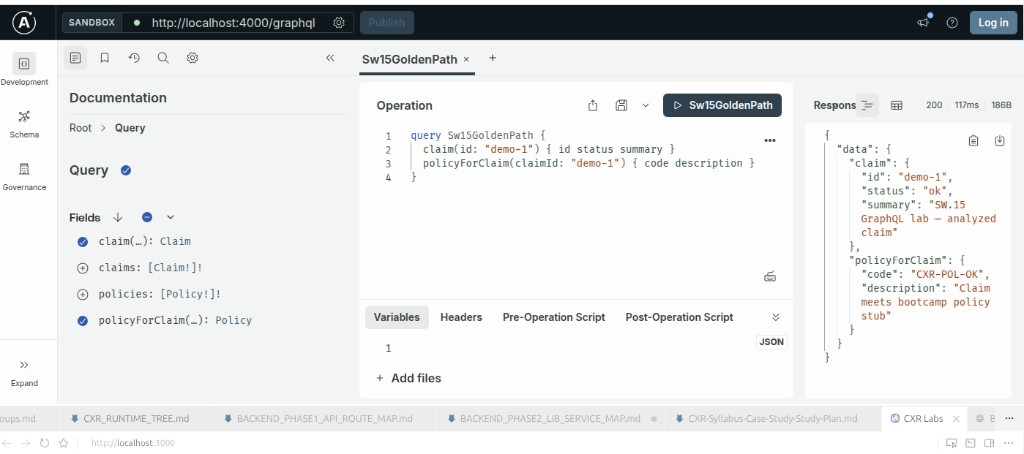
\includegraphics[width=0.92\textwidth]{../evidence/SW15-graphql-sandbox-2026-05-31.png}
\caption{Apollo Sandbox --- \texttt{status: ok}, \texttt{CXR-POL-OK} (SW.15 evidence).}
\end{figure}

\end{document}
